%-*- coding: UTF-8 -*-  表明了文件的编码类型是UTF-8。
% gougu.tex  原文件的文件名。
% 勾股定理 %原文件的内容
\documentclass[UTF8]{ctexart} %表明文档类,这里是“中文的短文”,所以使用ctexart。并用[UTF8选项说明编码]
\usepackage{graphicx}
\usepackage{float}
\usepackage{amsmath}

\title{杂谈勾股定理}
\author{赵康}
\date{\today}
\newtheorem{thm}{定理}

\begin{document} %和后边的end{document}构成document环境,里边是论文的正文部分。
\bibliographystyle{plain} %声明参考文献的格式
\maketitle %必须要加上这个,否则title中的内容不显示。输出论文标题
\begin{abstract}
    这是一篇关于勾股定理的小短文 %这里在插入title后加入文章摘要
\end{abstract}
\tableofcontents %命令输出目录
\section{勾股定理在古代} %开始新的一节
西方称勾股定理为毕达哥拉斯定理,将勾股定理的发现归功于公元前 6 世纪的毕达哥拉斯学派\cite{kline}。
该学派得到一个法则,可以求出排除直角三角形三边的三元数组。毕达哥拉斯学派没有书面著作,
该定理的严格表述和证明见于欧几里得\footnote[1]{欧几里得,公元前 330——275 年}《几何原本》的命题 47:“直角三角形斜边上的正方形
等于两直角边上的两个正方形之和。”证明是用面积做的。


我国《周髀算经》载商高(约公元前 12 世纪)答周公问  %段前不用打空格,有空格自动忽略。latex会自动生成空格。
%使用空行分段,单个换行不会使文字另起一段,只是让源代码更易读。多个空行会使文字分段
%中文后边单个换行就相当于空格,英文里边空格就是一个空格
\begin{quote} %quote环境,将内容单独分行,增加缩紧和上下间距排印,以突出引用部分.
    \zihao{-5}\kaishu 勾广三,股修四,径隅五 %\zihao{} 是一个参数命令,-5 就是小五号;而\kaishu 则是没有参数命令,把字体切换为楷体。
\end{quote}
又载陈子(约公元前 7——6 世纪)答荣方问:
\begin{quote}
    \zihao{-5}\kaishu 若求邪至日者,以日下为勾,日高为股,勾股各自相乘,并而开方除之,得邪至日。
\end{quote}
都较古希腊更早。后者已经明确道出了勾股定理的一般形式。图\ref{fig:xiantu}是我国古代对勾股定理的一种证明\cite{shanggao}。
\begin{figure}[ht] %我们使用的figure环境,就是插入使用的浮动体环境。【ht】表示浮动体可以出现在环境周围的文本所在处
    \centering %\centering表示后边的内容居中。
    文本所在处
    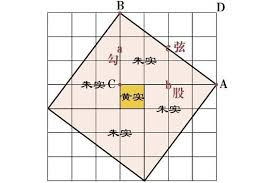
\includegraphics[scale=0.6]{xiantu.jpeg}
    \caption[short]{宋赵爽在《周髀算经》注中作的弦图(仿制),改图给出了勾股定理一个极具对称美的证明} %\caption命令给插入加上自动编号和标题
    \label{fig:xiantu} %\label命令给图形加一个标签,使用这个标签就可以在文章的其他地方引用\caption产生的编号
\end{figure}

\section{勾股定理的近代形式}%开始新的一节
勾股定理可以用现代语言描述如下:
\begin{thm}[勾股定理]
直角三角形斜边的平方等于两腰的平方和。


可以用符号语言表述为:这直角三角形ABC,其中 $\angle C = 90^\circ$,则有 
\begin{equation}
    \label{eq:gougu}
    AB^2 = AC^2 + BC^2
\end{equation}
\end{thm}
满足式\eqref{eq:gougu}的整数称为\emph{勾股数}。第一节所说的毕达哥拉斯学派得到的三元数组就是勾股数。下表列出了一些较小的勾股数
\begin{table}[H]
\begin{tabular}{|ccc|} %tabular 环境中有一个参数,里边声明了表格中列的模式。r、l、c表示靠右、靠左、居中,|表示要画的竖线。
\hline %横线的命令是hline,表格内部的表项用&连接。各个行之间用\\隔开
直角边$a$ & 直角边$b$ & 斜边$c$ \\
\hline
3 & 4 & 5 \\
5 & 12 & 13 \\
\hline
\end{tabular}%
\qquad %\qquad命令让我们把表格和公式并排 排开。\qquad 产生大约两个M的空白。
($a^2 + b^2 = c^2$)
\end{table}
    
\bibliography{math} %输出文献。

\end{document}
